
\documentclass[11pt]{article}
\usepackage[utf8]{inputenc}
\usepackage{float}
\restylefloat{table}
\usepackage{listings}
\lstset{
  basicstyle=\tiny
}

\usepackage{graphicx}
%Gummi|061|=)
\title{\textbf{NetInf. HTTP Protocol}}
\author{Backend/Frontend}
\date{}



\begin{document}

\maketitle
\clearpage
\tableofcontents
\clearpage

\section{Convergence Layer Specifications}
There are two different convergence layers that represent instantiations of the NetInf protocol, one being based on HTTP and the other on UDP.\\
For the second sprint of our project, our main focus will remain on the HTTP CL.

\subsection{HTTP Convergence Layer}
The HTTP CL is intended for use of the NetInf protocol in existing web infrastructures.
As you might recall there are three basic types of requests when using the NetInf protocol; Publish, Get and Search.
The following subsections will describe how these messages look within the HTTP CL instantiations of the NetInf protocol.
\\ \\
The HTTP CL assumes that the client knows the addresses of the HTTP server to which it will send requests.\\
NetInf HTTP responders MUST accept requests to the following paths:\\ \\
/netinfproto/get - for NetInf GET requests\\
/netinfproto/publish - for NetInf PUBLISH requests\\
/netinfproto/search - for NetInf SEARCH requests\\

\begin{figure}[H]
\centering
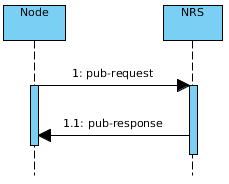
\includegraphics[width=0.5\textwidth]{seq_pub.png}
\caption{Flow of information for a publish request.}
\label{fig:sequence_get}
\end{figure}

\begin{figure}[H]
\centering
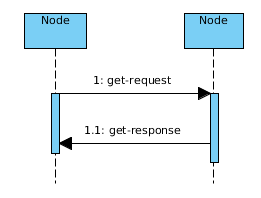
\includegraphics[width=0.5\textwidth]{seq_get.png}
\caption{Flow of information for a get request.}
\label{fig:sequence_get}
\end{figure}

\subsubsection{Publish request message}
\begin{table}[h]
\begin{tabular}{|l|l|}
\hline
$ Http form field$&$Comments$\\

\hline

URI&Usally an ni URI in the form of:\\
 &ni:///sha-256;644mOZ-DTu66fQt415\_kXE...?ct=text/plain\\
 &or locator.\\
\hline
msgid&a message identifier\\
\hline
loc 1&location one(for example the wifi-address)\\
\hline
.&.\\
\hline
.&.\\
\hline
loc n&location n(for example the bluetooth macaddress)\\
\hline
rform&"json" or "html". If rform is absent, the "json" value is assumed.\\
\hline
fullPut&If "fullPut" is absent, a "no" value is assumed.\\
 &if "fullPut" is set to "yes", "octets" must be present.\\
\hline
octets&Contains the file specification and the object octets.\\
\hline
ext&The value of "ext" MUST be a JSON object string and the value\\
 &of the "meta" item MUST be a subsidary object.\\
  &example:\\
  & \{"meta": \{ "mi1": .. \} \}\\
\hline
\end{tabular}
\caption{Publish Request Message}
\label{table:tab1}
\end{table}

A publish request message is sent from a node when that node wants to tell the network that they have something that they want to be able to distribute. Nodes does not distinguish if that specific publish is a completely new object or just want to register a copy of something they found in the network. The message is sent as a HTTP post and contains "key-" and "value"-like pairs, the exact content of these keys and values are found in table~\ref{table:tab1}.

\lstinputlisting[caption={Example Publish Request Headers},label=pub-example]{example-publish-request-headers.txt}

\subsubsection{Publish response message}
\begin{table}[H]
\begin{tabular}{|l|l|}
\hline
$JSON Key$&$Comments$\\

\hline

NetInf&version number of netinf\\
\hline
ni&Usally the "canonialized" form of the NDO as a URI in the ni scheme\\
 &(the URI without any netloc or query string fields). Example:\\
  &ni:///sha-256;644mOZ-DTu66fQt415\\
  &or locator.\\
\hline
msgid&the message identifier from the request\\
\hline
ts&Timestamp of the last publish\\
\hline
status&taken from the HTTP response, 203 in this case\\
\hline
ct&the MIME content type of the NDO content data.\\
 &(could be extracted from the ct within the ext from the request)\\
 &Empty string if not yet known.\\
 \hline
loc&a json-array containing the known locations.\\
\hline
\end{tabular}
\caption{Publish Response Message}
\label{table:tab2}
\end{table}
For publish, the HTTP response will contain an application/json or text/html response,depending on the value of rform in the publish request(remember that if rform was not present in the request json is the default).\\
A successfull response (HTTP response code 203) will be a application/json component that consists of a JSON object with the fields showed in table~\ref{table:tab2}.

\lstinputlisting[caption={Example PUB Response},label=pub-resp-example]{example-pub-response.json}

\subsubsection{GET request message}

\begin{table}[H]
\centering
\begin{tabular}{|l|l|}
\hline
$Http form field$&$Comments$\\

\hline

URI&Usally an ni URI in the form of:\\
 &ni:///sha-256;644mOZ-DTu66fQt415\_kXE...\\
 &or locator.\\
\hline
msgid&a message identifier\\
\hline
loc 1&location one(for example the wifi-address)\\
\hline
.&.\\
\hline
.&.\\
\hline
loc n&location n(for example the bluetooth macaddress)\\
\hline
ext&This field isn't used for anything at the moment\\
 &but exists for future use.\\
\hline
\end{tabular}
\caption{GET Request Message}
\label{table:tab3}
\end{table}

A GET request message is sent from a node when that node want to get something from the network. The message is sent as a HTTP post and contains "key-" and "value"-like pairs, the exact content of these keys and values are found in table~\ref{table:tab3}.

\lstinputlisting[caption={Example GET Request Headers},label=get-req-example]{example-request-header.txt}

\subsubsection{GET response message}
\begin{table}[H]
\centering
\begin{tabular}{|l|l|}
\hline
$JSON Key $&$Comments$\\

\hline

NetInf&version number of netinf\\
\hline
ni&Usally the "canonialized" form of the NDO as a URI in the ni scheme\\
 &(the URI without any netloc or query string fields). Example:\\
  &ni:///sha-256;644mOZ-DTu66fQt415\\
    &or locator.\\
\hline
msgid&the message identifier from the request\\
\hline
ts&Timestamp of the last publish\\
\hline
status&taken from the HTTP response\\
 &200 in case of affiliated data and content\\
 &203 in case of only affiliated data\\
\hline
ct&the MIME content type of the NDO content data.\\
 &Empty string if not yet known.\\
\hline
\end{tabular}

\label{table:tab4}
\caption{GET Response Message}
\end{table}
For a successful GET response(HTTP response code 203 or 200) the HTTP response will contain either an application/json(if no object is returned) or a multipart/mixed response with exactly two body parts, the first being the application/json and the second being the actual object(with whatever MIME type is appropriate), depending on if the node receiving the request has the NDO requested or not.\\

\lstinputlisting[caption={Example GET Response, multi-part, octets present},label=get-resp-multi-part]{example-get-response-multi-part.txt }

\lstinputlisting[caption={Example GET Response, no octects},label=get-resp-json]{example-get-no-octets.json }



\subsubsection{Search Message}
Postponed to later in the project.\\

\subsubsection{Search response Message}
Postponed to later in the project.\\

\end{document}
